\documentclass[12pt]{article}
\usepackage{amssymb,amsmath}
\usepackage[unicode=true]{hyperref}
\usepackage[margin=2cm]{geometry}
\usepackage{tikz}
\usepackage{pgfplots}
\usetikzlibrary{shapes}
\usetikzlibrary{calc}
\usetikzlibrary{arrows.meta}
\usetikzlibrary{spy}
\usepackage[europeanresistors]{circuitikz}
\usepackage[most]{tcolorbox}
\tikzset{component/.style={draw,thick,circle,fill=white,minimum size =0.75cm,inner sep=0pt}}
\usepackage{siunitx}
\usepackage{subfig}


\usepackage{framed}

\title{Topics in Electricity and Magnetism}
\author{Paul Druce}
\date{}

\begin{document}
\maketitle

\section{Charge}\label{the-basics}

So electricity is all about \emph{Charge}. What it is, how it moves and what it's useful for. 
Charge is the name given to a weird property that amber (the material) has when it was rubbed with wool by the Ancient Greeks\footnote{Fun fact, the word electric comes from the Greek word \emph{elektron} which means amber.}. 
The Greeks noticed that the amber would attract other small object such as fur and repel other pieces of amber that has been rubbed with fur. It was said that amber acquired a net \emph{charge}. 
It was also noticed (much later in time) that if you rubbed glass with silk it would attract the silk - it gained a charge. However, amber (plastic works too) that has been rubbed with fur would then attract this glass rod, not repel it. 
This lead people to believe there were two distinct types of electric charge and Benjamin Franklin (1706-1790) started calling these \emph{positive} and \emph{negative}. 
Hence the phrase \emph{``opposites attract"} or more formally:
\begin{quote}
Two positive charges or two negative charges repel each other. A
positive and a negative charge attract each other.
\end{quote}


The majority of electrical inventions and developments were built using this level of knowledge. The notion of a particle nature to charge was not suspected until much later. A weird result of this time delay between experimentation with electricity and a fundamental understanding has lead to some \emph{conventions} that you may find irritating\footnote{One of these conventions is that it is the positive charge that moves. This means that you understanding of electrons flowing with often butt up against this convention. So be aware.}. We now know, that was happening in the process of rubbing various
materials with other materials is that \textbf{electrons} are being
transferred. 
The electron is a \emph{fundamental particle}\footnote{A fundamental particle is just on object which, as far as we know, has no sub-structure. Electrons, neutrinos, muons, taus etc are all fundamental. It was once though that protons and neutrons were fundamental particles, however it was discovered that they are made up of quarks.} which we say has charge \(-e\). 
The electron is taken to define the fundamental
unit of charge. 

There are particles with positive charge also. The proton is the classic example, which has a charge of $+e$. It should be noted that there are other particles with other values of positive and negative charge. For instance, there are two types of quarks, one with charge $+2/3e$ and another type with charge $-1/3 e$. The fractional values are purely based on the fact that we hold the electron as the unit of charge. As the quarks were discovered much more recently that the electron, the standard of charge was already well established.

However for practical purposes, as we rarely deal with small numbers of electrons, other (more appropriate) units of charge exists. 
The standard unit is that of \textbf{Coulombs}, which, if we were to measure the electrons charge in Coulombs it would be \(-e = -1.602176 \times 10^{-19}C\). An incredibly tiny value. 
For instance to make up -1 Coulombs of charge requires over 6 billion billion electrons\footnote{Prove to yourself that this value is roughly correct.}. A number so large that is makes no sense to imagine.  

The way the Coulomb is defined is in terms of macroscopic quantities.
Quantities that physicists in the previous centuries would have been able to measure and use.
% Now in real life we rarely deal with single electrons or even tens of electrons, we often deal with billions upon billions of them at a time.
% Rather than just saying that charge shall be measured in the terms of \(e\), we deal with Coulombs, \(C\), as in the value I've given for \(e\). 
A Coulomb is defined the be the amount of charge that passes a fixed point when a \emph{current} of 1 \emph{Ampere} flows for one second.
So what is current and what is an Ampere?
% \begin{description}
% \item[Question]
% \textbf{Basic Questions about charge}
% \end{description}

\section{Current}\label{current}

Current in terms of electricity is the motion of charge from one region to another. Just as in the sea current refers to motion of water from one place to another. 
However, current was defined and used to describe electricity well before we the particles that make up charge. 
So whats referred to as \emph{conventional current} is defined to be the flow of positive charge. 
Despite the fact that the positively charged objects (the atomic nuclei) don't move in conductors, and its the negatively charged electrons which flow.

This is someone confusing when you first see it, but what you have to
remember is that physics and especially electricity were studied well
before the 21st century. We have see that the Ancient Greeks were
investigating the basics of this phenomena, and it was until 1879 that
the notion of the electron was introduced and it wasn't discovered until 1897. To put this in perspective the electric motor was invented in the 1820s, that's 70 years earlier. So we had been using electricity for quite literally a lifetime before we started
fully understanding what was happening at the atomic level.

Back to current, so current, denoted by \(I\), is defined to be the
amount of charge passing a certain point per second.
\[I = \frac{\Delta Q}{ \Delta t}.\]
Current is measured in terms of \(Amperes\) or \(Amps\) for short. \(1\) ampere is defined to be one coulomb per second \footnote{The actual definition by SI is given in terms of forces between two parallel rods. In fact a lot of these units are potentially going to be \emph{redefined} in terms of \emph{fundamental constants}. For instance it has been proposed that the Coulomb be defined to be so that the electron has the exact value of \(-1.6021766208 \times 10^{-19}C\) for its charge.}.

% \begin{description}
% \item[Question]
% \textbf{Need basic question}
% \end{description}

\subsection{Drift Velocity}\label{drift-velocity}

Inside a conducting wire such as the copper wires that supply power to the plugs in your house. The motion of the electrons is not a smooth journey from the national grid\footnote{Appreciating where your electricity comes from is a hot topic at the moment. The main forms either being from coal and gas plants, that burn fossil fuels to create super-heated steam to turn turbines, or, renewable energy production such as solar panels, wind farms, tidal generators. Nuclear fission is also a procedure to produce energy, and arguably has the biggest controversy around it. You will learn about nuclear fission reactors within your A level physics course.} to your plug. They will move erratically, bouncing off the nuclei of the metal atoms. This chaotic motion means that despite the electrons moving very fast, it takes them a relatively long time to travel any macroscopic distance. We get a useful velocity by taking the average of the electron's velocity over some small time scale, we call this new velocity the \emph{drift velocity}. Note that this will be in the opposite direction to the current (due to electrons being negatively charged). 

\begin{figure}[h]
\centering
\begin{framed}
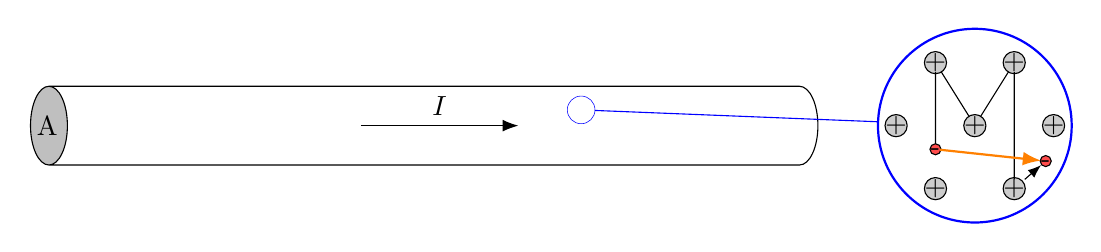
\begin{tikzpicture}
    \begin{scope}[spy using outlines={circle, magnification=7, size=5cm, connect spies}]
    \node (A) [cylinder, aspect=2, shape border rotate=180, draw,minimum height=10cm,minimum width=1cm,cylinder uses custom fill, cylinder end fill =gray!50, anchor=west] {};
    \node at (0.22,0) {A};
    \draw[-{Latex[length=2mm]}] ($(A.center)+(-1,0)$) to ($(A.center)+(1,0)$);
    \node[above] at (A.center) {$I$};
    \spy[blue,size=7em] on (7,0.2) in node (below) at (12,0);
    \end{scope}
    \foreach \x in {0,1}
        \draw[black, fill=gray!40,inner sep=0pt,outer sep=0pt] ($(below.center)+(-0.5+\x,0.8)$) circle[radius=4pt] node (nuclei1\x) {+};
    \foreach \x in {0,1,2}
        \draw[black, fill=gray!40,inner sep=0pt,outer sep=0pt] ($(below.center)+(-1+\x,0)$) circle[radius=4pt] node (nuclei2\x) {+};            
    \foreach \x in {0,1}
        \draw[black, fill=gray!40,inner sep=0pt,outer sep=0pt] ($(below.center)+(-0.5+\x,-0.8)$) circle[radius=4pt] node (nuclei3\x) {+};
    \draw[black, fill=red!70,inner sep=0pt,outer sep=0pt] ($(below.center)+(-0.5,-0.3)$) circle[radius=2pt] node (electron1) {-};
    \draw[black, fill=red!70,inner sep=0pt,outer sep=0pt ] ($(electron1)+(1.4, -0.15)$)
    circle[radius=2pt] node (electron2) {-};
    \draw[-Latex] (electron1) -- (nuclei10) --  (nuclei21) -- (nuclei11) -- (nuclei31) -- (electron2);
    \draw[thick, -Latex, color=orange] (electron1) to (electron2) node[font=\tiny,below,xshift=-2em,yshift=0.4em] {};
\end{tikzpicture}
\caption{The black line in the zoomed-in blue circle represents the true path the electron travels within the wire. The orange line is the average path the electron takes which we define to be equal to $v_d \cdot \Delta t$.}
\end{framed}
\end{figure}

The reason we are interested in this drift velocity is that it is helpful when talking about currents.
Imagine we have a cylindrical wire with cross section \(A\). 
In some small amount of time denoted \(\Delta t\), the electrons will move a length of \(v_d \cdot \Delta t\). 
Considering a section of the wire that is $v_d \Delta t$ long, assume there are $n$ electrons moving within it.
As each electron has a charge of \(-e\), and the wire has a cross sectional area of \(A\), we will have that the total charge that move through this section is given by \[\Delta Q  = +e (n\cdot A\cdot v_d \cdot \Delta t )\]. 
So the current is given by \[I = \frac{\Delta Q}{\Delta t} = e n A v_d\]


So why do electrons flow through wires? They can't always do that, otherwise I'd get electric shocks from every piece of metal. So what causes them to move? What have we assumed in the above figure? To explain the origin of this motion, we introduce the idea of \emph{potential differece}.

% \begin{description}
% \item[Question]
% \textbf{Need a question}
% \end{description}



\section{Potential Difference}\label{potential-difference}
A potential difference is what makes electricity flow, and it usually provided by
batteries or cells. These are an objects with a negative terminal
at one end and a positive terminal at the other, and so when its
connected via circuit it cause electrons to flow to even the charges. I
like to think of it in terms of hills and balls, a potential difference
sets up a hill with the high end being the negative terminal and bottom
of the hill being the positive terminal, and the battery as a sort of
lift/ elevator back up to the top of the hill. However, this is entirely
heuristic and shouldn't be relied on too heavily for calculations.

In physics, we say that a potential difference provides the energy to
cause charge to flow. So it measures the amount of energy needed to move
one Coulomb of charge between the two points your measuring. So letting
\(W\) denote the \emph{energy transferred} or \emph{work done} and let
\(Q\) be the amount of charge we have the formula for potential
difference as \[V = \frac{W}{Q}\] and its measured in \emph{Volts},
hence the letter \(V\). \(1\) Volt is defined potential difference
between two points that will give 1 Joule per Coulomb of charge that
passes through it.

An alternative way to think about this notion is to rearrange the
formula to give \[W = V \cdot Q.\] Which you can read as saying the
amount of energy to move a charge, \(Q\), through a potential difference
of \(V\) is given by the product of \(V\) and \(Q\).

% \begin{description}
% \item[Question]
% \textbf{need a question}
% \end{description}

\section{Resistance and
Resistivity}\label{resistance-and-resistivity}

The resistance of a material is way to tell how good a conductor it is.
For instance, copper has a very low resistance and wood has a very high
resistance. Resistance is defined to be the ratio of potential
difference across a sample of the material to the current flowing
through it. \[R = \frac{V}{I}\]

So if a material has a low resistance, then it means for a given voltage
it has a high current, and if a material has a high resistance then for
the same voltage the current would be much less.

The resistance of a material relies on its shape and size as well as
what its made of. To remove the shape and size dependance we can talk
about the \emph{resistivity} of a material. Which we can relate to the
resistance as follows: \[R = \frac{\rho L}{A}\] Where here \(\rho\) is
the resistivity, \(L\) is length of the material and \(A\) is the cross
sectional area. Basically, the longer the piece of material we have, the
higher its resistance regardless of what its made of\footnote{except for
  superconductors, but will get to that some other time}. The cross
sectional area you can think of how wide the wire is that we are
examining. Therefore the wider the wire, the lower resistance it will
have.

Resistance is measure in \textbf{Ohms} and is given the symbol
\(\Omega\). \(1\) Ohm is equal to \(1\) Volt per Ampere, i.e.
\(1\Omega = 1 V/ A\).

\subsection{Conductance and conductivity}\label{conductance-and-conductivity}
The conductivity of a material is the opposite of its resistance. It is a measure of how well electrons flow through the material. It is usually given the letter $G$ and is defined to be the \emph{reciprocal} of the resistance, i.e. $$G = {1\over R} = {I\over V}.$$
We can apply the same logic as above for the resistivity to a notion of \emph{conductivity}. Notice that 
$$G = {1 \over R} = {A \over \rho L},$$
so we define the conductivity as $\sigma = {1 \over \rho}$ so we have that 
$$G = {\sigma A \over L}$$

\subsection{Resistors and circuits}\label{resistors-and-circuits}

A resistor is a circuit device that is designed to have a certain
resistance between its ends. The ones we see in day to day life are
cylindrical and can range in value from \(0.01 \Omega \) to
\(10^7 \Omega \).

The symbol for a resistor are shown in Figure~\ref{fig:resistors}

\begin{figure}[h]
  \centering
\subfloat[][European]{
\centering
\begin{circuitikz} \draw
    (0,0) to[R] (2,0);
\end{circuitikz}}\qquad
\subfloat[][American]{
\begin{circuitikz}[american]\draw
    (0,0) to[R] (2,0);
\end{circuitikz}}
\caption{Circuit symbols for resistors}\label{fig:resistors}
\end{figure}

When we put resistors in series or parallel we can treat this system of resistors as one resistor with an effective resistance. And the effective resistance is calculated using various rules that we will state now and derive later on.

If we consider Figure~\ref{fig:seriesparallel:series}, we can ask ourselves is there a way to represent this circuit in the form of Figure~\ref{fig:effective}? The answer is yes, and the formula for the \emph{effective resistance}, $R_{\text{eff}}$, is given by
$$R_{\text{eff}} = R_1 + R_2 + R_3.$$

We can ask ourselves the same thing for Figure~\ref{fig:seriesparallel:parallel} and the answer is again yes and the formula for the effective resistance is given by
$$\frac{1}{R_{\text{eff}}} = \frac{1}{R_1}+ \frac{1}{R_2}+ \frac{1}{R_3}$$



\noindent\begin{figure}[t]
  \centering
  \begin{minipage}{0.4\textwidth}\centering
  \subfloat[][Resistors in series]{\label{fig:seriesparallel:series}
    \begin{circuitikz}\draw
      (0,0) node[circle,left]{a} to[R,color=red,l=$R_1$] (2,0) node[above] {x}
      (2,0) to[R,color=red,l=$R_2$] (4,0) node[circle,above] {y}
      (4,0) to[R,color=red,l=$R_3$] (6,0) node[right] {b}
      (6,0) to (6,2)
      (0,2) to[battery1,a^=$V_{\text{in}}$,i = $I$] (6,2)
      (0,2) to (0,0);
      \filldraw[fill=black] (0,0) circle (1pt);
      \filldraw[fill=black] (2,0) circle (1pt);
      \filldraw[fill=black] (4,0) circle (1pt);
      \filldraw[fill=black] (6,0) circle (1pt);
  \end{circuitikz}}
\end{minipage}~\hfil
\begin{minipage}{0.4\textwidth}\centering
  \subfloat[][Parallel resistors]{\label{fig:seriesparallel:parallel}
\begin{circuitikz} \draw
(0,1) to[short,-*] (1,1) node[below left] {d}
(1,1) -- (1,2)
(1,1) -- (1,0)
(1,2) to[R,l = $R_1$,color=red] (3,2)
(1,1) to[R,-,l=$R_2$,color=red] (3,1)
(1,0) to[R,l=$R_3$,color=red] (3,0)
(3,2) -- (3,1)
(3,0) to[short,-*] (3,1) node[below right] {e}
(3,1) -- (4,1) to (4,4)
(0,1) to (0,4) to[battery1,a^=$V_{\text{in}}$, i = $I$] (4,4)
;
\end{circuitikz}}
\end{minipage}
\caption{Circuits with resistors in series and parallel.  }~\label{fig:seriesparallel}
\end{figure}

\begin{figure}[b]
  \centering
  \begin{circuitikz}\draw
    (0,0) to[R,l_=$R_{\text{eff}}$] (4,0) to (4,2)
    (4,2) to[battery1, a^=$V_{\text{in}}$] (0,2) to (0,0);
  \end{circuitikz}
  \caption{What we want to convert the circuits in Figure\ref{fig:seriesparallel} into.}~\label{fig:effective}
\end{figure}

\subsection{Derivation of Series/Parallel Resistor formulas (not examinable, but worthwhile understanding)}

\underline{Series}

There are some key facts about the electromagnetic force that you need to know in order to derive the equations about. The first is that the electromagnetic force is a \emph{conservative} force. This means many things depending on what aspect of the EM force you want to examine. For us, it tells us that the work done to move a charge from one point to another, doesn't depending on the path taken. For instance in Figure~\ref{fig:seriesparallel:series}, if we move a charge from $a$ to $b$, the work done doesn't depending on whether we go through the cell or the resistors. It just depends on the distance between the two points. Now, we can ask ourselves, well what happens if we ask about the potential difference from point $a$ to point $a$, we can view this as the electron not moving, or by going all the way around the circuit. Well, the potential difference has to be zero. Which means that the potential differences across each component have to add up to zero.
If we label the potential difference between point $a$ and point $b$ by $V_{ab}$
Then we have the following formulas
$$V_{aa} = 0$$
and
$$V_{aa} =  V_{in} - (V_{ax} + V_{xy} + V_{yb}),$$
where I've labelled the cell as having a positive potential difference and the resistors as having a negative potential difference.
So we have that
\begin{equation}\label{eq:Vsum}V_{in} = V_{ax}+ V_{xy} + V_{yb}.\end{equation}

\emph{So the voltage provided by the cell is distributed between the components of a circuit}

Now if we again consider Figure~\ref{fig:seriesparallel:series}, we can use some basic physicaly intuition about current to arrive at the formulas for effective resistance of a series circuit. The core feature to notice, is that current is the amount of charge flowing past a point in the circuit. As the charges are the same sign (electrons are all negatively charged) they don't want to get bunched up in any one area. That means that the current at any point in a wire is the same. Resistors don't affect this rule, so the current at points $a,x,y,b$ has the same value. Because the charge can't go anywhere else. There is only one path for each electron to take.
So the current going through each resistor is the same as the current at point $a$, which we will call $I$.

Then using Ohm's Law: $V_i= I\cdot R_i$, where $i=1,2,3$ and represents the resistance and potential difference across the resistors $R_1, R_2, R_3$. Then using Equation~\ref{eq:Vsum} and that $V_{in} = I \cdot R_{\text{eff}}$, we get that:
\begin{align}
  V_{in} = I\cdot R_{\text{eff}} = I \cdot (R_1 + R_2 + R_3)
\end{align}
And so by dividing by $I$, we get the formula for resistors in series:
$$R_{\text{eff}} = R_1 + R_2 + R_3$$

\underline{Parallel}

To derive the formula for the parallel resistors, we again start with the same facts about the electromagnetic force. Using Figure~\ref{fig:seriesparallel:parallel} as our example and starting with the fact that the potential difference between two points doesn't depend on the path between those two points. So for instance, the potential difference between points $d$ and $e$ in Figure~\ref{fig:seriesparallel:parallel}, doesn't depend on whether you go through the cell or across the parallel resistors. So it's value should match that of the cell, $V_{in}$. This means that the potential difference across all of the resistors is equal to potential difference between $d$ and $e$, because of the path independence.

Next we examine the current across the circuit, imagine that across the cell we have a current of $I$. The current is a measure of how much charge flows past a point, and our charges aren't allowed to ``build up'' at any point on the circuit. That means the current flowing through point $d$, has to match that flowing through point $e$, no more, no less. So the amount of charge flowing through the resistors has to add up to the amount of charge flowing through $d$. If we label the current flowing through $R_1,R_2,R_3$ as $I_1, I_2, I_3$, the have the following expression
$$I_a = I_1 + I_2 + I_3$$

Then again using Ohm's law, we get that
$$I = \frac{V_{in}}{R_{\text{eff}}} = I_1 + I_2 + I_3 = V_{in}(\frac{1}{R_1}+\frac{1}{R_2}+\frac{1}{R_3})$$

Which by the eliminating the potential difference from the equation, we get that
$$\frac{1}{R_{\text{eff}}} = \frac{1}{R_1}+ \frac{1}{R_2}+ \frac{1}{R_3}$$


\section{Electromotive force}\label{electromotive-force}



Lets clear some things up right away. Electromotive force or \emph{EMF},
is not a force, its actually an \emph{energy-per unit charge} quantity
so its measured in \emph{volts}.

EMF is basically the potential difference a cell when it delivers no
current. So if you were to take a battery at home, and a voltmeter and
measure the voltage across the two terminal of the battery (assuming
that the battery has no \textbf{internal resistance} and the voltmeter
has no resistance) what you would be measuring is the EMF.\@ EMF is given the symbol $\mathcal{E}$

Batteries, solar cells, generators are all called \emph{sources of EMF}, as they provide the energy to cause a current to flow.

\subsection{Internal Resistance}

This viewpoint of EMF is an idealised one. In real life, the sources of EMF have some resistance of their own which impedes the conversion of the energy stored in the battery to the motion of the charges. This is called \emph{internal resistance} and is denoted by lower case $r$. If the source obeys Ohm's law, then the voltage across the terminals of the cells will measure a voltage of
\begin{equation}
  V_{ab} = \mathcal{E} - Ir \label{eq:EMF_PD}
\end{equation}

The current in the circuit attached the cell still obeys $V_{ab} = IR$, and so we can write the current as follows:

$$I = \frac{\mathcal{E}}{R+r}$$

So it's worth noting that if you are provided with an EMF and an internal resistance, you need to calculate the potential difference across the circuit by Equation~\eqref{eq:EMF_PD}, which will be difference to the EMF.


\section{Potential Dividing Circuits}
A potential dividing circuits (often just refered to as a potential divider) is any circuit that can produce a different ``output'' voltage that is a fraction of the ``input'' voltages. These circuits are typically fairly simple, with the simplest being two resistors in series:

\begin{center}
  \begin{circuitikz}\draw
    (0,2) to[R,l=$R_1$] (2,2) to[R,l=$R_2$] (4,2) to (4,3)
    to[battery1, a=$V_{in}$] (0,3) to (0,2)
    (0.1,2) to (0.1,1) to (1,1) node[component]{$V_{out}$} to (1.9,1) to (1.9,2);
  \end{circuitikz}
\end{center}

This is the sort of circuit you may be presented with. However, this isn't the most enlightening way to show you when we use potential dividers.

A more informative ciruit is given by:

\begin{center}
  \begin{circuitikz}\draw
    (0,0) to[R,l=$R_1$] (0,2)
    (0,0) to[R,l=$R_2$] (0,-2)
    (0,2) to[short,-o] (-1,2) node[above]{$V_{in}$}
    (0,-2) node[ground]{}
    (0,0) to[short,-o] (1.5,0) node[above]{$V_{out}$};
  \end{circuitikz}
\end{center}

In this circuit we have an input potential difference, which could be provided by the mains in your house for instance. And we then have a simple circuit which will change the output potential difference by connecting a resistor series between in the input wire and ground or neutral. As mains in the UK is $\SI{240}{\volt} $, and USB is typically $\SI{5}{\volt} $, these sorts of circuits will be used everyday.

If we consider the first circuits (the closed one) we can use Ohm's law to write a formula for $V_{out}$. Recalling that the current around the circuit is the same everywhere as we are dealing with a series circuit. We have that $I = \frac{V_{in}}{R_{tot}}$ and also $I = \frac{V_1}{R_1} = \frac{V_2}{R_2}$. So specifically we have that:
$$V_i = V_{in} \frac{R_i}{R_{tot}}. $$


\section{Kirchoff's Laws}
Not all circuits can be reduced so a simple square, some take on the forms such as this:
\begin{center}
  \begin{circuitikz}\draw
    (0,0) node[below]{c} to (2,0) node[below]{b} to (4,0) node[below]{d}
    (4,0) to[R] (4,2)
    (0,2) to[battery1] (0,0)
    (0,2) to (2,2)
    (2,2) node[above]{a} to[battery1] (2,0)
    (2,2) to (4,2);
    % (1,1) node[scale=4]{$\circlearrowright$}
    % (1,1) node{$l_1$}
    % (3,1) node[scale=4]{$\circlearrowright$}
    % (3,1) node{$l_2$};
  \end{circuitikz}
\end{center}

To help deal with these sorts of situations there are a set of rules called Kirchoff's Rules. Its a small set, consisting of only two rules. But there require some definitions.

\noindent\underline{Definition: Junction}\\
A junction is the meeting point of 3 lines.

So for instance, a and b are junctions, whereas c and d are not.

\noindent\underline{Definition: Loop}\\
A loop is any closed path within a circuit.


So to tackle this, start to label current directions on the circuit. We do this without knowing exactly how the current is flowing. But Kirchoffs Rules will give us negative values for the current if we have labelled them the wrong way around. So it doesn't matter.
So consider the following:
\begin{center}
  \begin{circuitikz}\draw
    (0,0) node[below]{c} to (2,0) node[below]{b} to (4,0) node[below]{d}
    (4,0) to[R,i<=$I_2$] (4,2)
    (0,2) to[battery1, i=$I_1$] (0,0)
    (0,2) to[short, i=$I_1$] (2,2)
    (2,2) node[above]{a} to[battery1,i=$I_3$] (2,0)
    (2,2) to[short, i=$I_2$] (4,2)
    (2,0) to[short, i=$I_1$] (0,0)
    (1,1) node[scale=4]{$\circlearrowright$}
    (1,1) node{$A$}
    (3,1) node[scale=4]{$\circlearrowright$}
    (3,1) node{$B$};
  \end{circuitikz}
\end{center}
here I've assumed some directions for the currents and i've labelled two of the three loops we have.
We then start to by examining the junctions. So looking at junction $a$, we have that $I_1 + I_3 - I_2 = 0$, because we say that a current is entering the junction if the arrow points to the junction, and if the arrow points away from the junction it's negative.


\end{document}
